% BEAMER ----
% This is just here so I know exactly what I'm looking at in Rstudio when messing with stuff.
\documentclass[12pt,ignorenonframetext,,aspectratio=149]{beamer}
\setbeamertemplate{caption}[numbered]
\setbeamertemplate{caption label separator}{: }
\setbeamercolor{caption name}{fg=normal text.fg}
\usepackage{lmodern}
\usepackage{amssymb,amsmath}
\usepackage{ifxetex,ifluatex}
\usepackage{fixltx2e} % provides \textsubscript
\ifnum 0\ifxetex 1\fi\ifluatex 1\fi=0 % if pdftex
  \usepackage[T1]{fontenc}
  \usepackage[utf8]{inputenc}
\else % if luatex or xelatex
  \ifxetex
    \usepackage{mathspec}
  \else
    \usepackage{fontspec}
  \fi
  \defaultfontfeatures{Ligatures=TeX,Scale=MatchLowercase}
  \newcommand{\euro}{€}
\fi
% use upquote if available, for straight quotes in verbatim environments
\IfFileExists{upquote.sty}{\usepackage{upquote}}{}
% use microtype if available
\IfFileExists{microtype.sty}{%
\usepackage{microtype}
\UseMicrotypeSet[protrusion]{basicmath} % disable protrusion for tt fonts
}{}

% Comment these out if you don't want a slide with just the
% part/section/subsection/subsubsection title:
\AtBeginPart{
  \let\insertpartnumber\relax
  \let\partname\relax
  \frame{\partpage}
}
\AtBeginSection{
  \let\insertsectionnumber\relax
  \let\sectionname\relax
  \frame{\sectionpage}
}
\AtBeginSubsection{
  \let\insertsubsectionnumber\relax
  \let\subsectionname\relax
  \frame{\subsectionpage}
}

\setlength{\emergencystretch}{3em}  % prevent overfull lines
\providecommand{\tightlist}{%
  \setlength{\itemsep}{0pt}\setlength{\parskip}{0pt}}
\setcounter{secnumdepth}{0}

\title{Globalization}
\subtitle{DPR 190}
\author{Miles D. Williams}
\date{}


%% Here's everything I added.
%%--------------------------

\usepackage{graphicx}
\usepackage{rotating}
%\setbeamertemplate{caption}[numbered]
\usepackage{hyperref}
\usepackage{caption}
\usepackage[normalem]{ulem}
%\mode<presentation>
\usepackage{wasysym}
%\usepackage{amsmath}


% Get rid of navigation symbols.
%-------------------------------
\setbeamertemplate{navigation symbols}{}

% Optional institute tags and titlegraphic.
% Do feel free to change the titlegraphic if you don't want it as a Markdown field.
%----------------------------------------------------------------------------------
\institute{Data for Political Research}

% \titlegraphic{\includegraphics[width=0.3\paperwidth]{\string~/Dropbox/teaching/clemson-academic.png}} % <-- if you want to know what this looks like without it as a Markdown field.
% -----------------------------------------------------------------------------------------------------



% Some additional title page adjustments.
%----------------------------------------
\setbeamertemplate{title page}[empty]
%\date{}
\setbeamerfont{subtitle}{size=\small}

\setbeamercovered{transparent}

% Some optional colors. Change or add as you see fit.
%---------------------------------------------------
\definecolor{clemsonpurple}{HTML}{522D80}
 \definecolor{clemsonorange}{HTML}{F66733}
\definecolor{uiucblue}{HTML}{003C7D}
\definecolor{uiucorange}{HTML}{F47F24}





% Some optional color adjustments to Beamer. Change as you see fit.
%------------------------------------------------------------------
\setbeamercolor{frametitle}{fg=clemsonpurple,bg=white}
\setbeamercolor{title}{fg=clemsonpurple,,bg=white}
\setbeamercolor{local structure}{fg=clemsonpurple,}
\setbeamercolor{section in toc}{fg=clemsonpurple,bg=white}
% \setbeamercolor{subsection in toc}{fg=clemsonorange,bg=white}
\setbeamercolor{footline}{fg=clemsonpurple!50, bg=white}
\setbeamercolor{block title}{fg=clemsonorange,bg=white}


\let\Tiny=\tiny


% Sections and subsections should not get their own damn slide.
%--------------------------------------------------------------
\AtBeginPart{}
\AtBeginSection{}
\AtBeginSubsection{}
\AtBeginSubsubsection{}

% Suppress some of Markdown's weird default vertical spacing.
%------------------------------------------------------------
\setlength{\emergencystretch}{0em}  % prevent overfull lines
\setlength{\parskip}{0pt}


% Allow for those simple two-tone footlines I like.
% Edit the colors as you see fit.
%--------------------------------------------------
\defbeamertemplate*{footline}{my footline}{%
    \ifnum\insertpagenumber=1
    \hbox{%
        \begin{beamercolorbox}[wd=\paperwidth,ht=.8ex,dp=1ex,center]{}%
      % empty environment to raise height
        \end{beamercolorbox}%
    }%
    \vskip0pt%
    \else%
        \Tiny{%
            \hfill%
		\vspace*{1pt}%
            \insertframenumber/\inserttotalframenumber \hspace*{0.1cm}%
            \newline%
            \color{clemsonpurple}{\rule{\paperwidth}{0.4mm}}\newline%
            \color{clemsonorange}{\rule{\paperwidth}{.4mm}}%
        }%
    \fi%
}

% Various cosmetic things, though I must confess I forget what exactly these do and why I included them.
%-------------------------------------------------------------------------------------------------------
\setbeamercolor{structure}{fg=blue}
\setbeamercolor{local structure}{parent=structure}
\setbeamercolor{item projected}{parent=item,use=item,fg=clemsonpurple,bg=white}
\setbeamercolor{enumerate item}{parent=item}

% Adjust some item elements. More cosmetic things.
%-------------------------------------------------
\setbeamertemplate{itemize item}{\color{clemsonpurple}$\bullet$}
\setbeamertemplate{itemize subitem}{\color{clemsonpurple}\scriptsize{$\bullet$}}
\setbeamertemplate{itemize/enumerate body end}{\vspace{.6\baselineskip}} % So I'm less inclined to use \medskip and \bigskip in Markdown.

% Automatically center images
% ---------------------------
% Note: this is for ![](image.png) images
% Use "fig.align = "center" for R chunks

\usepackage{etoolbox}

\AtBeginDocument{%
  \letcs\oig{@orig\string\includegraphics}%
  \renewcommand<>\includegraphics[2][]{%
    \only#3{%
      {\centering\oig[{#1}]{#2}\par}%
    }%
  }%
}

% I think I've moved to xelatex now. Here's some stuff for that.
% --------------------------------------------------------------
% I could customize/generalize this more but the truth is it works for my circumstances.

\ifxetex
\setbeamerfont{title}{family=\fontspec{serif}}
\setbeamerfont{frametitle}{family=\fontspec{serif}}
\usepackage[font=small,skip=0pt]{caption}
 \else
 \fi

% Some random stuff now...
% ------------------------

\usepackage{tikz}

\newcommand{\shrug}[1][]{%
\begin{tikzpicture}[baseline,x=0.8\ht\strutbox,y=0.8\ht\strutbox,line width=0.125ex,#1]
\def\arm{(-2.5,0.95) to (-2,0.95) (-1.9,1) to (-1.5,0) (-1.35,0) to (-0.8,0)};
\draw \arm;
\draw[xscale=-1] \arm;
\def\headpart{(0.6,0) arc[start angle=-40, end angle=40,x radius=0.6,y radius=0.8]};
\draw \headpart;
\draw[xscale=-1] \headpart;
\def\eye{(-0.075,0.15) .. controls (0.02,0) .. (0.075,-0.15)};
\draw[shift={(-0.3,0.8)}] \eye;
\draw[shift={(0,0.85)}] \eye;
% draw mouth
\draw (-0.1,0.2) to [out=15,in=-100] (0.4,0.95);
\end{tikzpicture}}

% header includes go last.


% Okay, and begin the actual document...

\begin{document}
\frame{\titlepage}

\hypertarget{globalization}{%
\section{Globalization}\label{globalization}}

\begin{frame}{Globalization}
\protect\hypertarget{globalization-1}{}
\begin{centering}

What is \textit{globalization}?

\end{centering}
\end{frame}

\begin{frame}{Globalization}
\protect\hypertarget{globalization-2}{}
\begin{centering}

\textbf{Globalization} usually is a term used to describe increasing \textit{cross-border} interconnections across the globe.

\end{centering}
\end{frame}

\begin{frame}{Globalization}
\protect\hypertarget{globalization-3}{}
\begin{centering}

How can we \textit{measure} globalization?

\end{centering}
\end{frame}

\begin{frame}{Globalization}
\protect\hypertarget{globalization-4}{}
\begin{centering}

A common way to measure globalization is \textit{trade}.

\end{centering}
\end{frame}

\hypertarget{when-did-globalization-begin}{%
\section{When did globalization
begin?}\label{when-did-globalization-begin}}

\begin{frame}{When did globalization begin?}
\protect\hypertarget{when-did-globalization-begin-1}{}
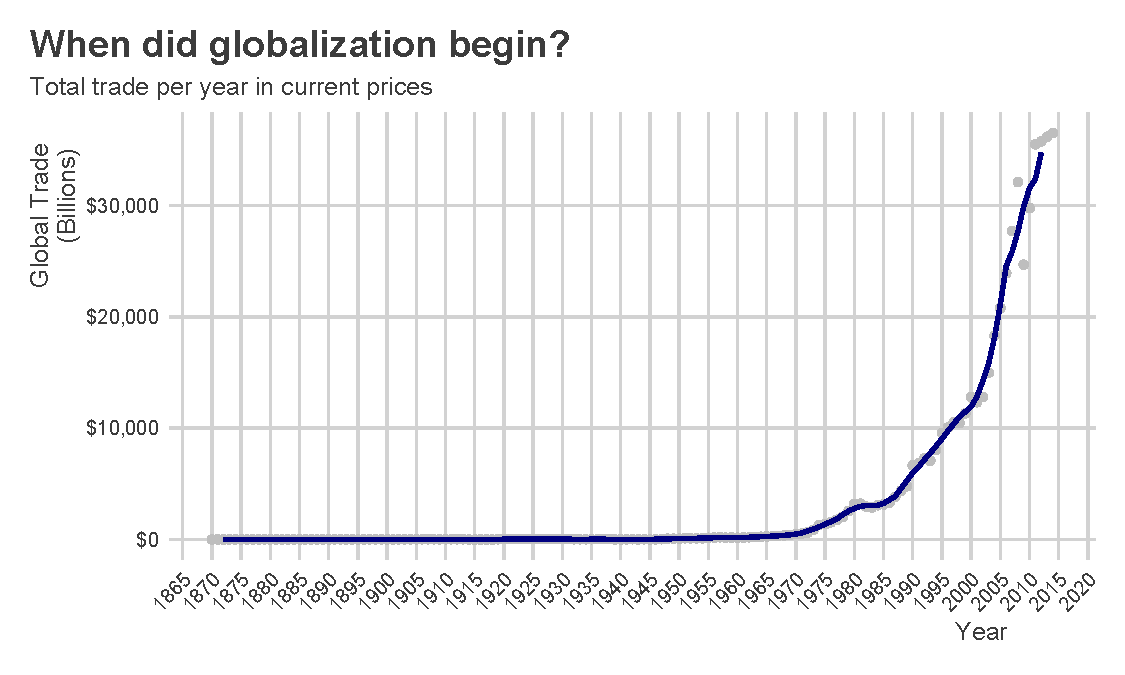
\includegraphics[width=0.9\linewidth]{05_slides_files/figure-beamer/unnamed-chunk-1-1}
\end{frame}

\begin{frame}{When did globalization begin?}
\protect\hypertarget{when-did-globalization-begin-2}{}
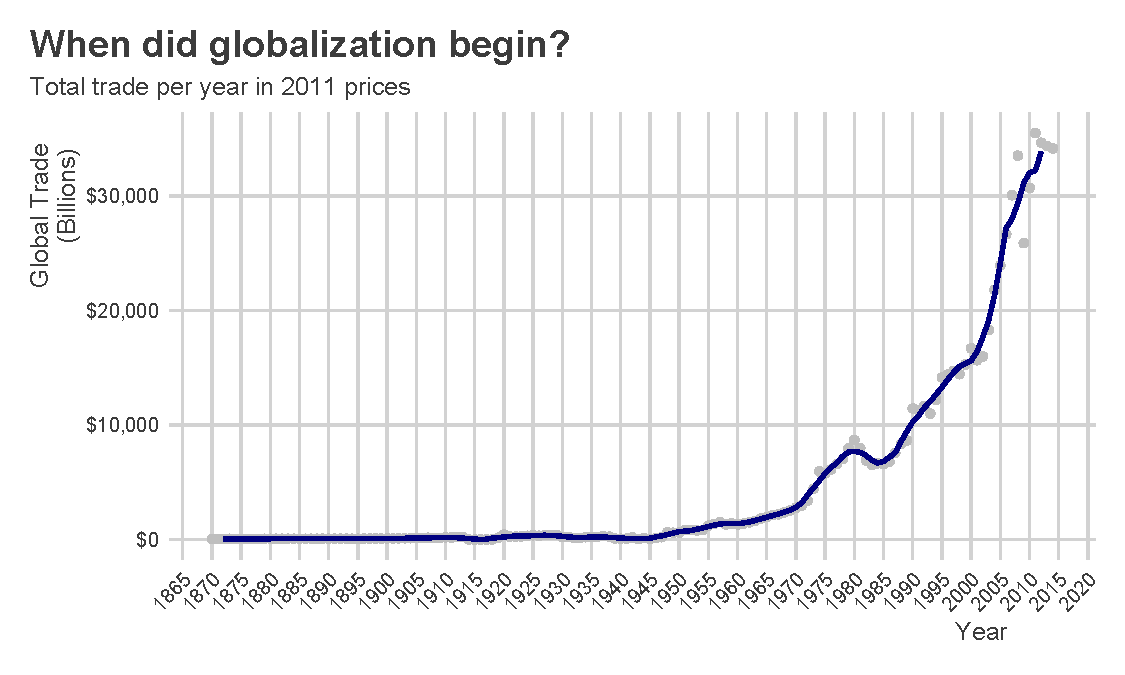
\includegraphics[width=0.9\linewidth]{05_slides_files/figure-beamer/unnamed-chunk-2-1}
\end{frame}

\begin{frame}{When did globalization begin?}
\protect\hypertarget{when-did-globalization-begin-3}{}
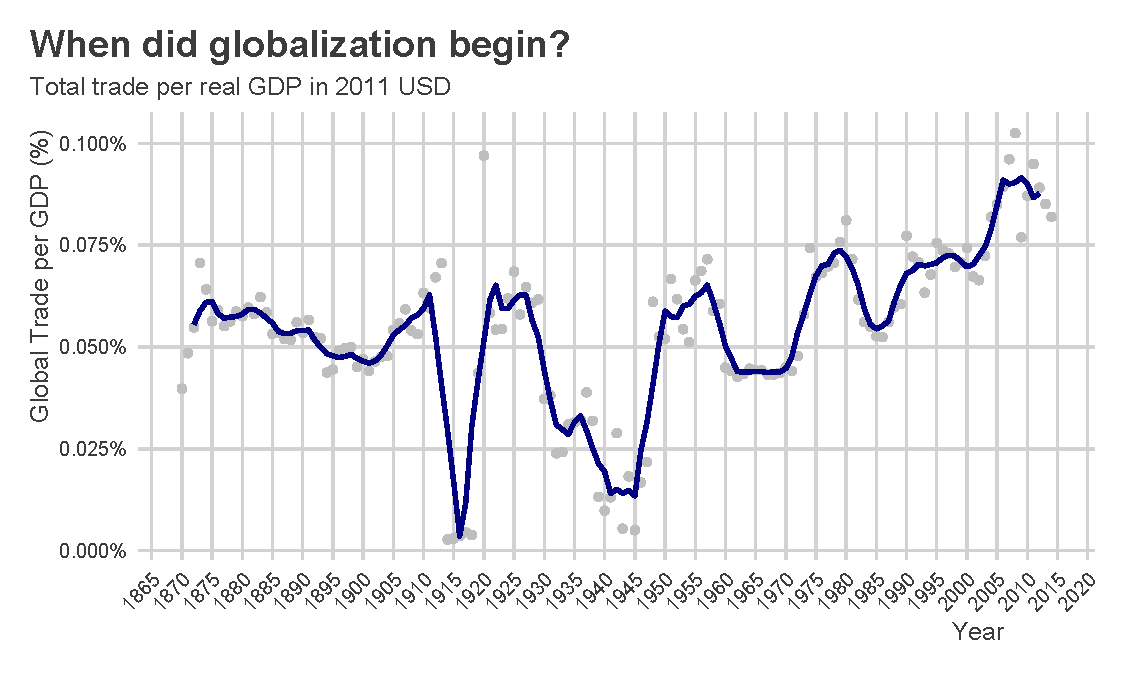
\includegraphics[width=0.9\linewidth]{05_slides_files/figure-beamer/unnamed-chunk-3-1}
\end{frame}

\hypertarget{how-global-is-globalization}{%
\section{How global is
globalization?}\label{how-global-is-globalization}}

\begin{frame}{How global is globalization?}
\protect\hypertarget{how-global-is-globalization-1}{}
\begin{itemize}
\tightlist
\item
  A key part of globalization is the idea that growing cross-border
  interconnections are \emph{global}.
\item
  Does this seem right to you?
\item
  How could we check?
\end{itemize}
\end{frame}

\begin{frame}{How global is globalization?}
\protect\hypertarget{how-global-is-globalization-2}{}
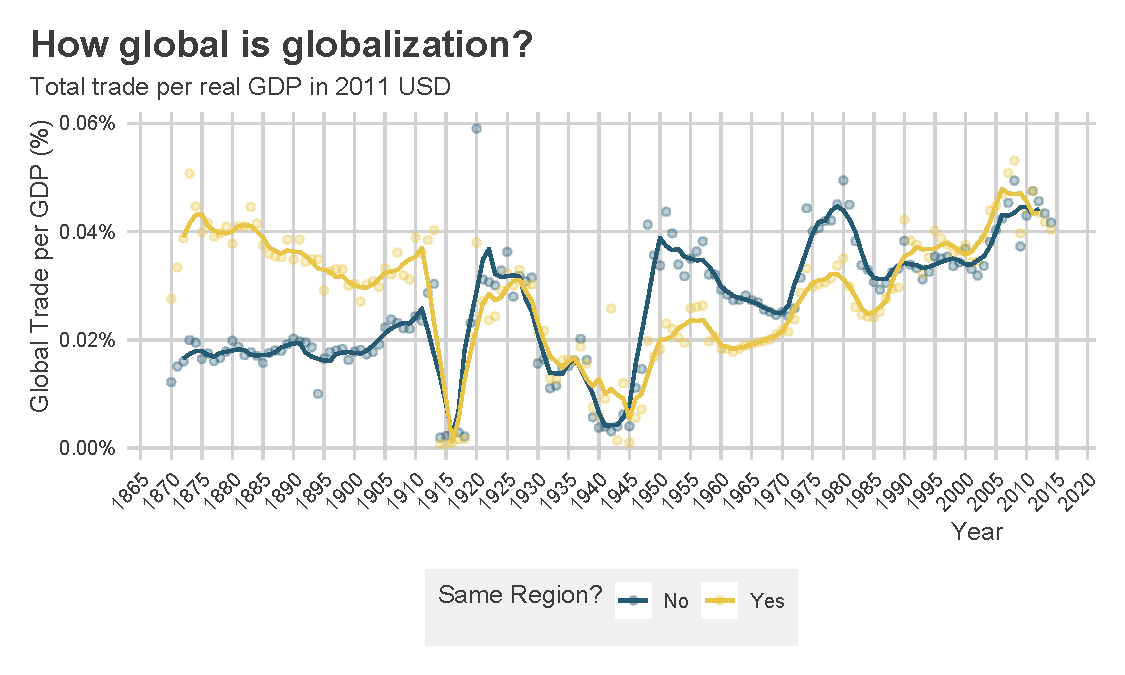
\includegraphics[width=0.9\linewidth]{05_slides_files/figure-beamer/unnamed-chunk-4-1}
\end{frame}

\begin{frame}{How global is globalization?}
\protect\hypertarget{how-global-is-globalization-3}{}
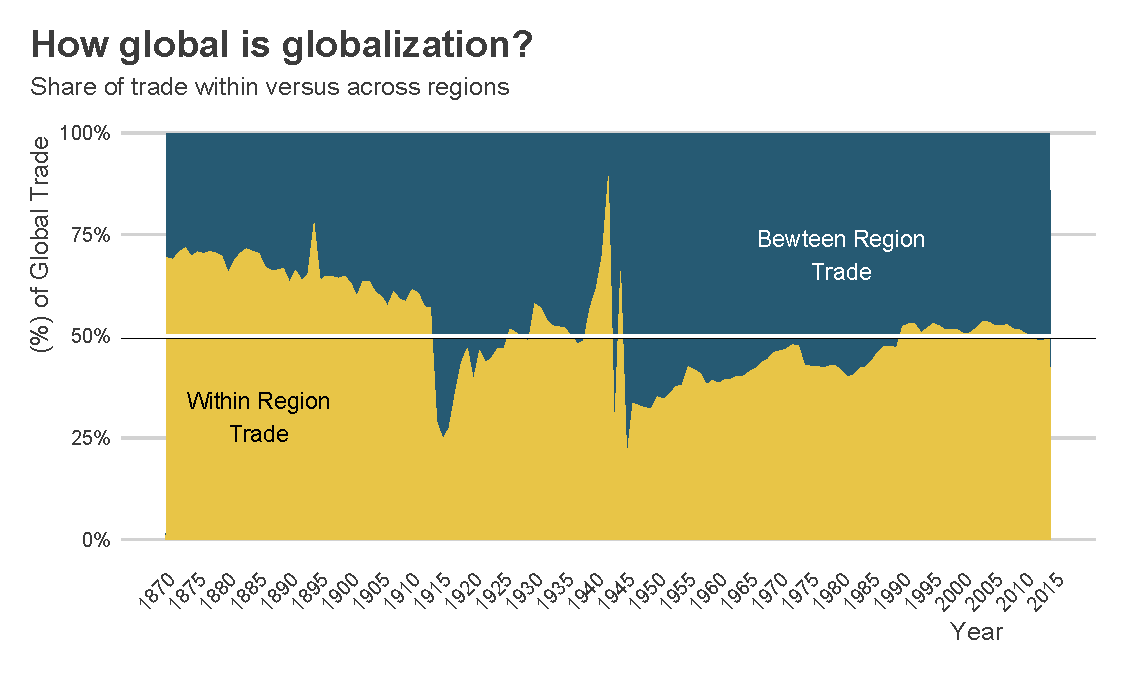
\includegraphics[width=0.9\linewidth]{05_slides_files/figure-beamer/unnamed-chunk-5-1}
\end{frame}

\begin{frame}{How global is globalization?}
\protect\hypertarget{how-global-is-globalization-4}{}
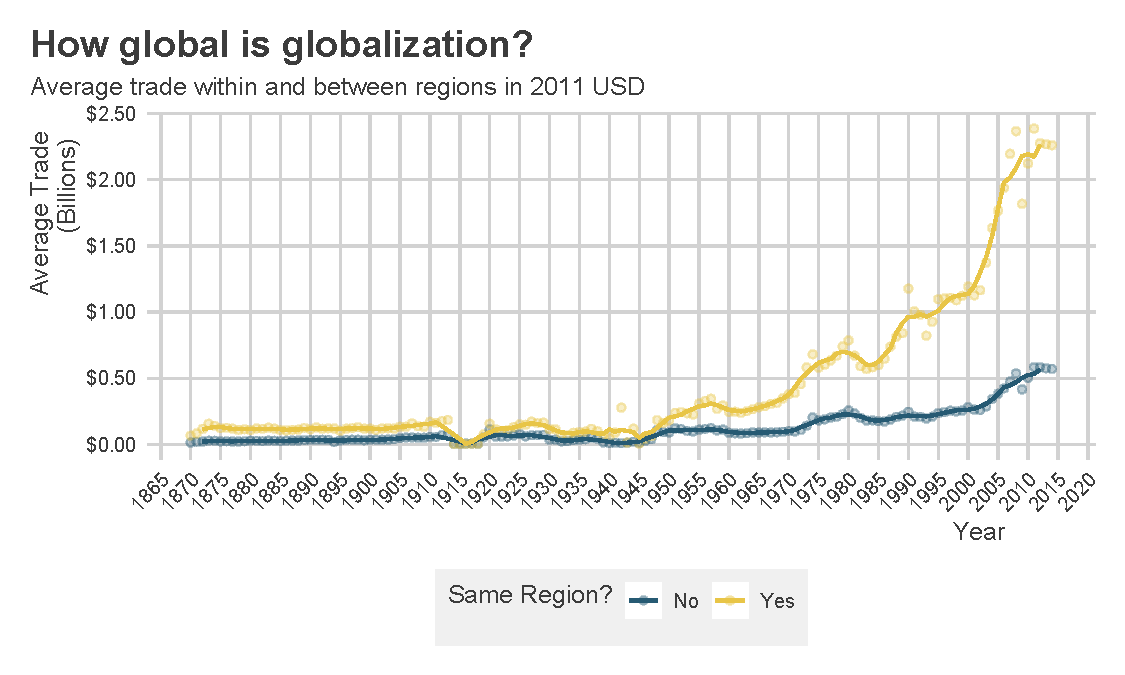
\includegraphics[width=0.9\linewidth]{05_slides_files/figure-beamer/unnamed-chunk-6-1}
\end{frame}

\begin{frame}{How global is globalization?}
\protect\hypertarget{how-global-is-globalization-5}{}
\begin{itemize}
\tightlist
\item
  Cross-border connections have been growing.
\item
  But these cross-border connections remain disproportionately
  \emph{regional} rather than \emph{global}.
\item
  Do you think this conclusion would be the same if we tried to measure
  globalization a different way?
\end{itemize}
\end{frame}

\hypertarget{next-time}{%
\section{Next Time}\label{next-time}}

\begin{frame}{Next Time}
\protect\hypertarget{next-time-1}{}
Henry Farrell and Abraham Newman, ``Chained to Globalization'' and
``Will the Coronavirus End Globalization as we Know It?''
\end{frame}


\section[]{}
\frame{\small \frametitle{Table of Contents}
\tableofcontents}
\end{document}
